%!TEX root = ../dissertation_vkslm.tex

\chapter{Proposed Method}\label{ch:method}




Although a simple static signature can be generated linking the points of the dynamic trajectory, additional dynamic information could be used to enrich the static signature. This addition is expected to lead more realistic and more discriminative images. Figure \ref{fig_approach} gives an overview of the proposed approach. In this section, we describe our proposed approach. First, the dataset used to train our model is described. Afterwards, we describe how the data was preprocessed. Finally, the CNN model is detailed. 

\begin{figure}[!htb]
\centering
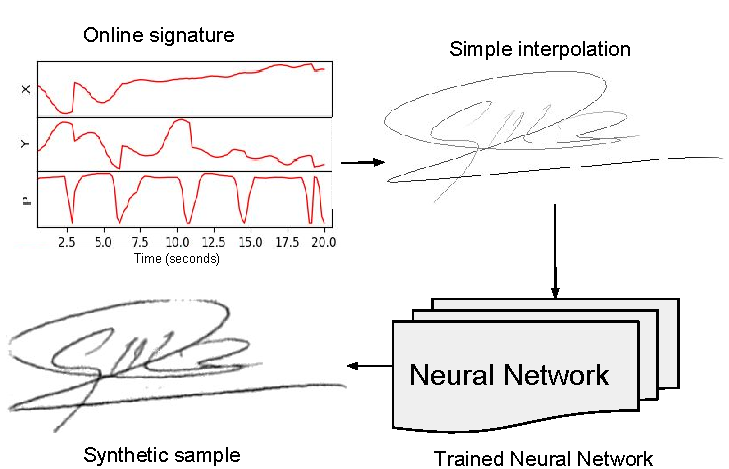
\includegraphics[width=6.5in]{method}
% where an .eps filename suffix will be assumed under latex, 
% and a .pdf suffix will be assumed for pdflatex; or what has been declared
% via \DeclareGraphicsExtensions.
\caption{The proposed approach diagram and an example of the synthetic signature generation.}
\label{fig_approach}
\end{figure}

\section{Training Dataset}
The neural network was trained using the data from the IRONOFF \cite{viard1999ireste} dataset, this database contains on-line manuscripts mapped to the corresponding static handwriting sample. It contains 1000 digitized documents in English and French written by 700 different writers.

\section{Preprocessing}
%Copy and paste
The neural networks expect inputs of a fixed size, where signatures vary significantly in
shape (in BiosecurID, they range from small signatures of size 153x258 to large signatures of size 819x1137 pixels). In order to have a fixed size, we first normalize the images to the largest image size, by padding the images with
white background. In this case, we centered the signatures in
a canvas of size 840x1360 pixels, aligning the center of mass
of the signature to the center of the image, similar to previous
approaches in the literature, e.g. \cite{pourshahabi2009offline}. We then rescaled the
images to 383x150 pixels. This size was chosen to be large enough to keep
details from the pen strokes in the manuscript, while still small
enough to enable to train on the GPU.

Besides resizing the images to a standard size, we also
performed the following pre-processing steps:
\begin{itemize}
\item Inverted the images: we inverted the images so that the white background corresponded to pixel intensity
0. 
\item Normalized the input: we normalized the input to the
neural network by dividing each pixel by the standard
deviation of all pixel intensities. We do not normalize the data to have mean 0 (another common pre-processing step) since we want the
background pixels to be zero-valued.
\item Interpolation: The on-line sequences ($x_{t}, y_{t}, p_{t}$) are linearly interpolated using Bresenham's line algorithm to obtain 8-connected sequences.
\end{itemize}

Figure \ref{fig_ironoff} shows an example of the preprocessed input and the ground truth that are fed to the neural network during training phase.


\begin{figure}[!htpb]
\centering
 \subfloat[input]{
\includegraphics[width=2.0in]{input-ironoff}} 
\hspace*{0.5in} % separation between the subfigures
\subfloat[ground truth] {
\includegraphics[width=2.0in]{gt-ironoff}}
\caption{Preprocessed data used during the training phase. (a) is the interpolated on-line sample, used as input and (b) is the expected prediction from the neural network, the ground truth. } \label{fig_ironoff}
\end{figure}



\section{Neural Network model}

Our model is based on the concept of autoassociative memory \cite{jensen1996physiologically}, \cite{weinberger2004specific}, commonly known as autoencoders. Autoencoders are normally used to reduce high-dimensional data into a low-dimensional code to later reconstruct the data from the compressed code, i.e., the desired output is the same of the input pattern \cite{kramer1991nonlinear}, \cite{hinton2006reducing}. In our case, instead of expect the output to be the same as the input, our Neural Network model is fed with the interpolated on-line sample and we expect the respective off-line sample on the output, i.e. the input is the dynamic information and the desired output is the static manuscript.

We use an architecture based on the Convolutional Autoencoder \cite{masci2011stacked}. The expectation is that by learning to transform between on-line information to off-line manuscripts, the network will learn convolution filters that are relevant to synthesize off-line signatures based the on-line sample.

\begin{table}[htb]
\ABNTEXfontereduzida
\centering
\label{cnn-arch}
  \begin{tabular}{cc}
  \toprule
  Layer        & Size \\
   \midrule \midrule
  Convolution           & 16x3x3        \\ \midrule
  Convolution           & 32x3x3        \\ \midrule
  Convolution           & 32x3x3        \\ \midrule
  Convolution           & 64x3x3        \\ \midrule
  Transpose Convolution & 64x3x3        \\ \midrule
  Transpose Convolution & 32x3x3        \\ \midrule
  Transpose Convolution & 32x3x3        \\ \midrule
  Transpose Convolution & 16x3x3        \\ \bottomrule
   
  \end{tabular}

\caption{ Summary of the CNN Layers}
\end{table}


For the purpose of replicating our experiment,
we provide a full list of the parameters used in our tests. Table \ref{cnn-arch} lists the definition of the Convolutional Autoencoder layers. For convolution and
transpose convolution layers, we list the size as NxHxW where N is the
number of filters, H is the height and W is the width of the
convolution and transpose convolution windows, respectively. For every layer we use a stride (the distance between applications of the convolution operation) of 2x2, and we pad the input for every layer with 0  evenly left and right. We use Leaky Rectified Linear Units (LReLUs) as the activation function for all convolutional layers. The weights of the model are initialized using the technique proposed by Glorot and Bengio \cite{glorot2010understanding}, and the biases to 0. We trained the model with Adam optimizer to minimize the minimum squared error (MSE) loss for 100 epochs, using a learning rate of 0.001, and mini-batches of size 16. The network was trained
using the library Tensorflow, and took around 72h to train on a GTX 670 GPU.
